\documentclass[14pt,a4paper]{extarticle}
\usepackage{fontspec}
\setmainfont{times.ttf}[Path=C:/Windows/Fonts/,BoldFont=timesbd.ttf,ItalicFont=timesi.ttf,BoldItalicFont=timesbi.ttf]
\setmonofont{consola.ttf}[Path=C:/Windows/Fonts/,BoldFont=consolab.ttf,ItalicFont=consolai.ttf,BoldItalicFont=consolaz.ttf]
\newfontfamily\cyrillicfonttt{cour.ttf}[Path=C:/Windows/Fonts/,BoldFont=courbd.ttf,ItalicFont=couri.ttf,BoldItalicFont=courbi.ttf]
\usepackage{polyglossia}
\setdefaultlanguage{russian}
\setotherlanguage{english}
\usepackage[left=30mm,right=15mm,top=20mm,bottom=20mm]{geometry}
\usepackage{setspace}
\onehalfspacing
\usepackage{indentfirst}
\setlength{\parindent}{1.25cm}
\setlength{\parskip}{0pt}
\usepackage{amsmath,amssymb,array,tabularx,longtable}
\usepackage{float}
\usepackage{graphicx}
\usepackage{listings}
\usepackage{caption}
\usepackage{tocloft}
\usepackage{titlesec}
\usepackage{fancyhdr}
\usepackage{hyperref}
\usepackage{multirow}
\hypersetup{unicode=true,colorlinks=false,pdfborder={0 0 0},linkbordercolor={0 0 0}}
\urlstyle{same}
\captionsetup{labelsep=endash,font=normalsize}
\captionsetup[figure]{name=Рисунок}
\captionsetup[table]{name=Таблица}
\captionsetup[table]{justification=raggedright,singlelinecheck=false,margin=0pt}
\captionsetup[lstlisting]{justification=raggedright,singlelinecheck=false,margin=5pt}
\renewcommand{\lstlistingname}{Листинг}
\renewcommand{\contentsname}{СОДЕРЖАНИЕ}
\renewcommand{\cftsecleader}{\cftdotfill{\cftdotsep}}
\renewcommand{\cfttoctitlefont}{\hfill\bfseries\large}
\renewcommand{\cftaftertoctitle}{\hfill}
\titleformat{\section}{\bfseries\large}{\thesection}{0.5em}{}
\titleformat{\subsection}{\bfseries}{\thesubsection}{0.5em}{}
\titlespacing*{\section}{1.25cm}{0pt}{1em}
\titlespacing*{\subsection}{1.25cm}{1em}{0.6em}
\pagestyle{fancy}
\fancyhf{}
\fancyfoot[C]{\thepage}
\renewcommand{\headrulewidth}{0pt}
\setlength{\headheight}{17pt}
\lstdefinestyle{gocode}{
  language=C++,
  basicstyle=\ttfamily\footnotesize,
  keywordstyle=\mdseries,
  columns=fullflexible,
  keepspaces=true,
  showstringspaces=false,
  breaklines=true,
  frame=single,
  framerule=0.3pt,
  xleftmargin=3mm,
  xrightmargin=3mm,
  aboveskip=0.6em,
  belowskip=0.6em
}
\lstset{style=gocode}
\newcommand{\structhead}[1]{\clearpage\phantomsection\addcontentsline{toc}{section}{#1}\begin{center}\bfseries #1\end{center}\vspace{0.5em}}
\newcommand{\conclusion}[1]{\par\medskip\noindent\hspace*{\parindent}\textbf{Вывод}\par\indent #1\par}


\numberwithin{equation}{section}
\setlength{\emergencystretch}{2em}
\newcommand{\fig}[3]{\begin{figure}[H]\centering
\includegraphics[width=\textwidth,height=0.73\textheight,keepaspectratio]{figures/#1.pdf}
\caption{#2}\label{#3}\end{figure}}
\newcommand{\srcitem}[1]{\item #1}
\begin{document}
\begin{titlepage}
\thispagestyle{empty}
\noindent\begin{minipage}[c]{0.16\textwidth}

\includegraphics[width=\linewidth]{b_logo.jpg}
\end{minipage}\hfill
\begin{minipage}[c]{0.82\textwidth}\centering\small\bfseries
Министерство науки и высшего образования Российской Федерации\\
Федеральное государственное автономное образовательное учреждение\\
высшего образования\\
«Московский государственный технический университет имени Н.~Э.~Баумана\\
(национальный исследовательский университет)»\\
(МГТУ им. Н.~Э.~Баумана)
\end{minipage}
\par\vspace{0.5em}\noindent\rule{\textwidth}{2pt}\par\vspace{1.5em}
\noindent ФАКУЛЬТЕТ \underline{«Информатика и системы управления»}\\[1em]
{\small\noindent КАФЕДРА \underline{«Программная инженерия»}}
\vspace{2.2cm}
\begin{center}
\bfseries\Large Лабораторная работа № 2\\[0.3em]
по дисциплине «Анализ алгоритмов»
\end{center}
\vspace{2.2cm}
\noindent\textbf{Тема} \underline{Сравнительный анализ алгоритмов умножения матриц}\\[1em]
\noindent\textbf{Студент} \underline{Понарин А.~А.}\\[1em]
\noindent\textbf{Группа} \underline{ИУ7-55Б}\\[1em]
\noindent\textbf{Преподаватели} \underline{Волкова Л.~Л., Строганов Д.~В.}
\vfill
\begin{center}Москва, 2026\end{center}
\end{titlepage}
\clearpage
\pagenumbering{arabic}
\setcounter{page}{2}


\renewcommand{\contentsname}{СОДЕРЖАНИЕ}
\tableofcontents
\structhead{ВВЕДЕНИЕ}
Цель работы — провести сравнительный анализ алгоритмов умножения матриц.

Для достижения поставленной цели необходимо решить следующие задачи:
\begin{enumerate}
\item описать классический алгоритм умножения матриц, алгоритм Винограда и его оптимизированный вариант;
\item разработать схемы алгоритмов и оценить их трудоёмкость и затраты памяти;
\item реализовать алгоритмы на языке C++ и проверить их корректность;
\item выполнить массированные замеры процессорного времени при одинаковых условиях;
\item сравнить результаты для чётных и нечётных размеров и установить, согласуются ли замеры с теоретическими оценками.
\end{enumerate}
Оформление отчёта выполнено с учётом ГОСТ 7.32--2017~[1].

\clearpage\section{Аналитическая часть}
\subsection{Постановка задачи}
Даны матрицы $A\in\mathbb{Z}^{m\times n}$ и $B\in\mathbb{Z}^{n\times q}$. Требуется получить матрицу $C=AB\in\mathbb{Z}^{m\times q}$:
\begin{equation}\label{eq:classic}
c_{ij}=\sum_{k=0}^{n-1}a_{ik}b_{kj},\quad 0\le i<m,\quad 0\le j<q.
\end{equation}
Число столбцов первой матрицы должно совпадать с числом строк второй. В программе размеры ограничены диапазоном от 1 до 2000, элементы — диапазоном от $-10^6$ до $10^6$. Вычисления выполняются в знаковых 64-разрядных целых числах. Для этих ограничений переполнение отсутствует: модуль результата не превосходит $2\cdot10^{15}$, а грубая верхняя граница промежуточной суммы Винограда составляет $6\cdot10^{15}<2^{63}-1$.

\subsection{Классический алгоритм}
Матрица результата заполняется нулями. Для каждой пары индексов $i,j$ во внутреннем цикле по $k$ к $c_{ij}$ прибавляется произведение $a_{ik}b_{kj}$. Порядок циклов реализации — $i,j,k$. Алгоритм применим к прямоугольным матрицам; значения элементов не влияют на число итераций.

\subsection{Алгоритм Винограда}
Метод Винограда основан на преобразовании скалярного произведения~[2]. Для двух соседних слагаемых справедливо тождество
\begin{equation}
xy+uv=(x+v)(u+y)-xu-yv.
\end{equation}
Положим $d=\lfloor n/2\rfloor$, $r=n\bmod2$. Вычислим вспомогательные множители:
\begin{equation}\label{eq:factors}
R_i=\sum_{k=0}^{d-1}a_{i,2k}a_{i,2k+1},\qquad
H_j=\sum_{k=0}^{d-1}b_{2k,j}b_{2k+1,j}.
\end{equation}
Тогда произведение определяется выражением
\begin{equation}\label{eq:win}
\begin{split}
c_{ij}={}&-R_i-H_j+\sum_{k=0}^{d-1}
(a_{i,2k}+b_{2k+1,j})\cdot{}\\
&\cdot(a_{i,2k+1}+b_{2k,j})+r\,a_{i,n-1}b_{n-1,j}.
\end{split}
\end{equation}
Последнее слагаемое вычисляется только при нечётном $n$. Для $n=1$ суммы пар пусты, и результат целиком даёт коррекция. Множитель $R_i$ используется во всех столбцах строки, а $H_j$ — во всех строках столбца. За счёт этого число умножений сокращается.

\subsection{Оптимизированный алгоритм Винограда}
Используется та же формула~\eqref{eq:win}, но изменена организация вычислений:
\begin{enumerate}
\item чётная граница $e=n-n\bmod2$ и признак нечётности вычисляются один раз;
\item индекс внутреннего цикла увеличивается на 2, обращения $2k$ заменены обращениями $k$;
\item множители и элементы результата накапливаются в локальных скалярных переменных; запись в массив выполняется после накопления;
\item коррекция нечётного размера включена в вычисление текущего элемента, отдельный проход по результату не нужен.
\end{enumerate}
Это оптимизация реализации; арифметическая формула и асимптотический порядок трудоёмкости сохраняются.
\conclusion{Рассмотрены три алгоритма решения одной задачи. Алгоритм Винограда уменьшает число умножений ценой дополнительных сложений и двух массивов множителей. Нечётное число общих измерений требует коррекции.}

\clearpage\section{Конструкторская часть}
\subsection{Схемы алгоритмов}
На рисунках~\ref{fig:class}--\ref{fig:optfac} приведены схемы алгоритмов. Парные блоки с одинаковой буквой обозначают границы цикла; при пустом диапазоне тело пропускается. Входные данные проверяются до вычислений.
\begin{figure}[H]\centering
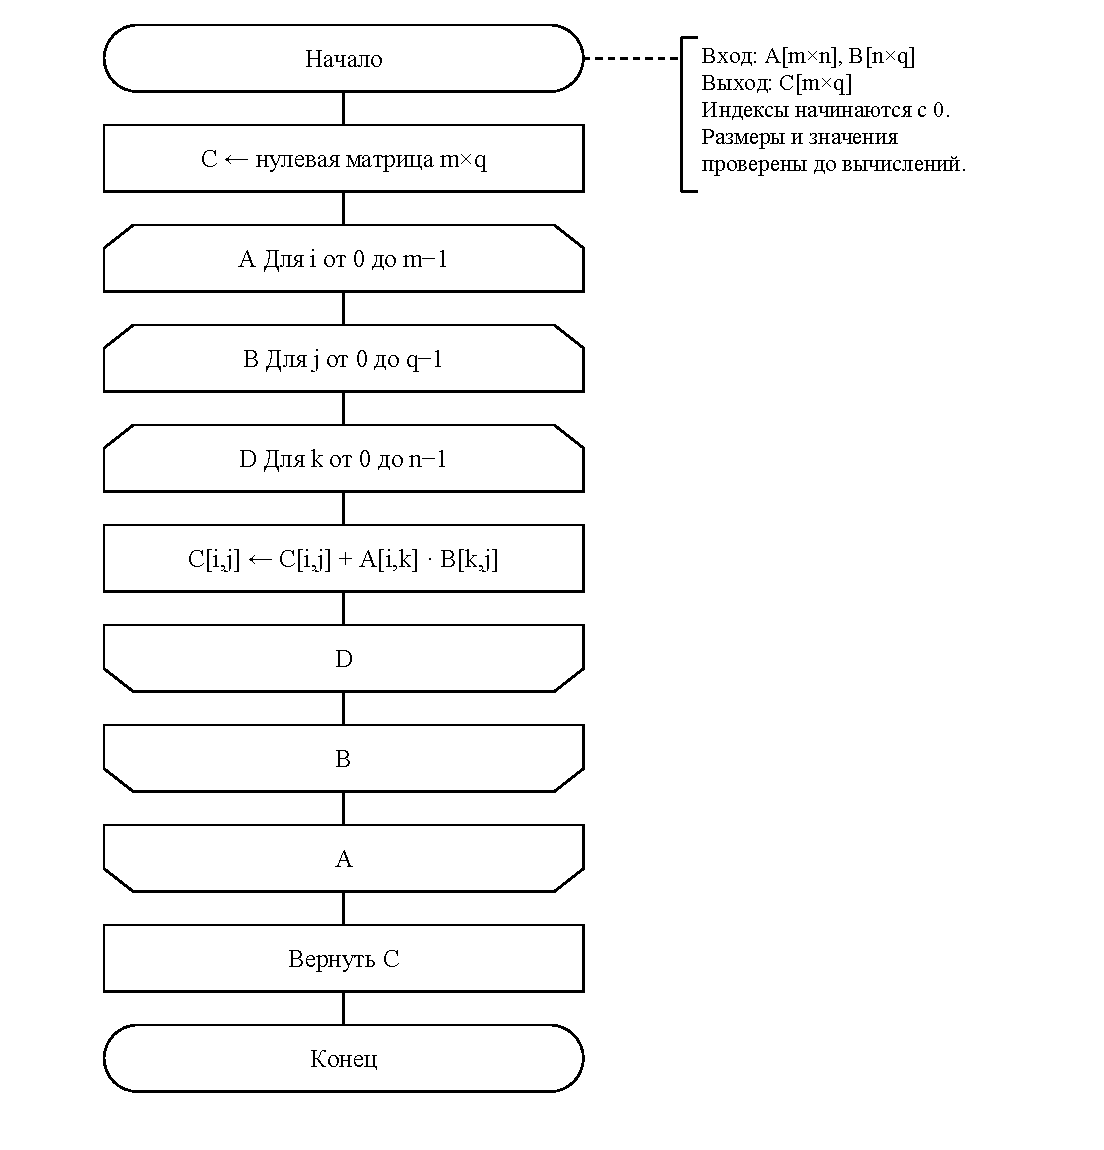
\includegraphics[width=\textwidth,height=0.65\textheight,keepaspectratio]{figures/classical.pdf}
\caption{Классический алгоритм умножения матриц}\label{fig:class}\end{figure}
\clearpage
\fig{winograd}{Алгоритм Винограда}{fig:win}
\clearpage
\fig{factors}{Вычисление множителей алгоритма Винограда}{fig:fac}
\clearpage
\fig{correction}{Коррекция результата при нечётном числе общих измерений}{fig:cor}
\clearpage
\fig{optimized}{Оптимизированный алгоритм Винограда}{fig:opt}
\clearpage
\fig{optimized_factors}{Оптимизированное вычисление множителей}{fig:optfac}

\subsection{Модель трудоёмкости}
Обозначим через $M$ число умножений элементов матриц, через $S$ — число сложений, вычитаний и унарных изменений знака элементов. Сложению и вычитанию приписывается стоимость $\alpha$, умножению — $\mu$, где $\alpha,\mu>0$. Арифметическая трудоёмкость равна
\begin{equation} F=\alpha S+\mu M. \end{equation}
Начальное заполнение массива нулями, проверки размеров и значений, операции над индексами, управление циклами и выделение памяти в этой модели не считаются арифметикой элементов матриц. Их влияние на полный алгоритм оценивается отдельно. Модель не отождествляется с количеством машинных инструкций или временем в секундах.

\subsection{Трудоёмкость классического алгоритма}
Тело внутреннего цикла выполняется $mnq$ раз и содержит одно умножение и одно сложение с текущей суммой, включая первое сложение с нулём. Поэтому
\begin{equation}M_{\text{кл}}=mnq,\qquad S_{\text{кл}}=mnq,\qquad
F_{\text{кл}}=(\alpha+\mu)mnq.\end{equation}
Для квадратных матриц порядка $N$ получаем $F_{\text{кл}}=(\alpha+\mu)N^3$. Организация циклов не зависит от значений элементов: при фиксированных размерах лучший и худший случаи совпадают по числу операций.

\subsection{Трудоёмкость алгоритма Винограда}
Вычисление множителей требует $(m+q)d$ умножений и столько же сложений. На каждый элемент результата приходятся две операции для $-R_i-H_j$, $d$ умножений и $3d$ сложений в основном цикле. При нечётном $n$ дополнительно выполняются одно умножение и одно сложение на элемент. Следовательно,
\begin{equation}
M_{\text{В}}=(m+q)d+mq(d+r),
\end{equation}
\begin{equation}
S_{\text{В}}=(m+q)d+mq(3d+2+r),
\end{equation}
\begin{equation}\label{eq:fw}
\begin{split}
F_{\text{В}}={}&(\alpha+\mu)(m+q)d+{}\\
&+mq\bigl((3\alpha+\mu)d+2\alpha+(\alpha+\mu)r\bigr).
\end{split}
\end{equation}
Для квадратных матриц и чётного $N$ формула принимает вид
\begin{equation}
F_{\text{В}}=\frac{3\alpha+\mu}{2}N^3+(3\alpha+\mu)N^2.
\end{equation}
При нечётном $N$, с учётом $d=(N-1)/2$, имеем
\begin{equation}
F_{\text{В}}=\frac{3\alpha+\mu}{2}N^3+
\frac{5\alpha+3\mu}{2}N^2-(\alpha+\mu)N.
\end{equation}
Для фиксированных размеров лучший и худший случаи также совпадают по числу операций. При одинаковых $m,q,d$ переход от $n=2d$ к $n=2d+1$ добавляет $mq$ умножений и $mq$ сложений.

\subsection{Трудоёмкость оптимизированного варианта}
Число арифметических операций над элементами совпадает с алгоритмом Винограда: $M_{\text{опт}}=M_{\text{В}}$, $S_{\text{опт}}=S_{\text{В}}$. Изменения относятся к индексам и обращениям к памяти. В исходном варианте выражение $2k$ встречается в телах циклов $(2m+2q+4mq)d$ раз, в оптимизированном — ни разу. Это количество записанных выражений в исходном коде, а не гарантия такого же числа машинных умножений: компилятор может преобразовать их в обоих вариантах.

Число записей в $C$ в основном вычислении уменьшается с $mq(d+1)$ до $mq$; коррекция нечётного случая не требует отдельного прохода. Множители также накапливаются в скалярах. Это объясняет возможность ускорения при одинаковой арифметической трудоёмкости.

Все реализации дополнительно проверяют элементы за $O(mn+nq)$, инициализируют результат за $O(mq)$ и выполняют служебные операции циклов. Полная трудоёмкость каждого алгоритма составляет $\Theta(mnq)$ для положительных размеров; для квадратных матриц — $\Theta(N^3)$.

Если положить $\alpha=\mu=1$, то для чётного $N$ получаются $F_{\text{кл}}=2N^3$ и $F_{\text{В}}=2N^3+4N^2$. Следовательно, само уменьшение числа умножений не доказывает ускорения в модели равных стоимостей. При $\mu>\alpha$ ведущий коэффициент Винограда меньше. Реальное время зависит также от компилятора и памяти и требует измерения.

\subsection{Оценка памяти}
Матрицы хранятся построчно в одномерных массивах элементов типа \texttt{int64\_t}. Полезные данные входа занимают $8(mn+nq)$ байт, результата — $8mq$ байт. Дополнительные массивы Винограда занимают $8(m+q)$ байт. Оценки не включают постоянные накладные расходы объектов контейнеров и распределителя памяти.
\begin{table}[H]\centering
\caption{Сравнение трудоёмкости и дополнительной памяти}\label{tab:theory}
\small\begin{tabularx}{\textwidth}{|X|c|c|}\hline
Алгоритм & Время, квадратные матрицы & Память без входа и выхода\\\hline
Классический & $\Theta(N^3)$ & $O(1)$\\\hline
Винограда & $\Theta(N^3)$ & $8(m+q)+O(1)$ байт\\\hline
Оптимизированный & $\Theta(N^3)$ & $8(m+q)+O(1)$ байт\\\hline
\end{tabularx}\end{table}
При учёте результата дополнительная память составляет $\Theta(mq)$ для классического алгоритма и $\Theta(mq+m+q)$ для вариантов Винограда. Для квадратных матриц все три оценки равны $\Theta(N^2)$.

\subsection{Требования к программе}
Программа должна обеспечивать ручной ввод и генерацию матриц, выбор любого из трёх алгоритмов, получение произведения прямоугольных матриц, проверку диапазонов и повтор ввода при ошибке. Отдельные режимы должны выполнять автоматические тесты и воспроизводимые замеры с сохранением результатов в CSV. Вычисления выполняются последовательно, в одном потоке.
\conclusion{Разработаны схемы алгоритмов, получены формулы арифметической трудоёмкости и оценки памяти. Оптимизации не меняют кубический порядок; для их практической оценки необходим эксперимент.}

\clearpage\section{Технологическая часть}
\subsection{Средства реализации}
Использован язык C++17 и компилятор GCC 14.2.0 (MSYS2 UCRT64). Из стандартной библиотеки применены контейнер \texttt{std::vector}, генератор \texttt{std::mt19937}, средства ввода-вывода и работы с файлами. Для замеров в Windows выбрана функция \texttt{GetProcessTimes}~[3].

В файлах \texttt{algorithms.hpp} и \texttt{algorithms.cpp} определены матрица, проверка допустимости данных и три алгоритма. В \texttt{main.cpp} размещены меню, тесты и измерительный стенд. Файл \texttt{CMakeLists.txt} задаёт сборку и тест CTest. Сборка измеряемой версии:
\begin{lstlisting}[language={},caption={Команда сборки программы}]
g++ -std=c++17 -O2 -Wall -Wextra -Wpedantic main.cpp algorithms.cpp -o matrix_lab.exe
\end{lstlisting}
\subsection{Реализация алгоритмов}
В листингах~\ref{lst:cl}--\ref{lst:opt} приведён код из поставляемого файла реализации. Функция \texttt{validate} проверяет совместимость размеров, структуру хранения и допустимость элементов; одинаковая проверка присутствует во всех трёх алгоритмах.
\lstinputlisting[firstline=21,lastline=30,caption={Классический алгоритм},label={lst:cl}]{algorithms.cpp}
\clearpage
\lstinputlisting[firstline=32,lastline=56,caption={Алгоритм Винограда},label={lst:win}]{algorithms.cpp}
\clearpage
\lstinputlisting[firstline=58,lastline=87,caption={Оптимизированный алгоритм Винограда},label={lst:opt}]{algorithms.cpp}

\subsection{Измерение процессорного времени}
Реальное время — длительность интервала между началом и концом операции по часам; оно включает ожидание и периоды, когда процесс не исполняется. Процессорное время учитывает выполнение потоков процесса на процессоре. Для однопоточной программы оно исключает время вытеснения другими процессами, но не устраняет влияние частоты процессора и подсистемы памяти.

По официальной документации Microsoft, \texttt{GetProcessTimes} возвращает накопленное время исполнения потоков процесса в пользовательском режиме и режиме ядра; значения представлены в 100-наносекундных единицах~[3]. Их сумма используется как процессорное время. Единица представления не означает фактическую точность таймера в 100 нс.
\lstinputlisting[firstline=27,lastline=42,caption={Получение процессорного времени процесса},label={lst:timer}]{main.cpp}
Значения времени чтения CSV, генерации входных матриц и проверки результатов в измеряемый интервал не входят. В него входят вызов алгоритма, проверка допустимости матриц, выделение и освобождение памяти результата и множителей, вычисление произведения и запись одного элемента в наблюдаемую переменную. Это измерение полной функции, а не изолированного арифметического ядра.

\subsection{Тестирование}
Автоматические проверки сопоставляют результат всех трёх реализаций с ожидаемым произведением. Для случайных матриц используется отдельная реализация по сумме внешних произведений с порядком циклов $k,i,j$. В таблице~\ref{tab:tests} приведены группы проверок.
\begin{table}[H]\centering\caption{Функциональные проверки}\label{tab:tests}
\small\begin{tabularx}{\textwidth}{|p{1cm}|>{\raggedright\arraybackslash}X|>{\raggedright\arraybackslash}p{3.2cm}|}\hline
№ & Данные / условие & Ожидаемый результат\\\hline
1 & $A=\left(\begin{smallmatrix}1&2&3\\4&5&6\end{smallmatrix}\right)$, $B=\left(\begin{smallmatrix}7&8\\9&10\\11&12\end{smallmatrix}\right)$ & $\left(\begin{smallmatrix}58&64\\139&154\end{smallmatrix}\right)$\\\hline
2 & $A=(-3)$, $B=(7)$ & $(-21)$\\\hline
3 & Нулевые матрицы $3\times4$ и $4\times2$ & Нулевая $3\times2$\\\hline
4--5 & $A I$ и $I A$, $A$ размера $3\times3$ & $A$\\\hline
6 & $(1,-2,3)\cdot(4,5,-6)^T$ & $(-24)$\\\hline
7 & $(10^6,-10^6)\cdot(10^6,-10^6)^T$ & $(2\cdot10^{12})$\\\hline
8 & 1000 случайных наборов, $m,n,q\in[1,10]$ & Совпадение с эталоном\\\hline
9 & Нулевой размер и размер 2001 & Исключение\\\hline
10 & Несовместимые размеры, нарушенное хранение, элемент $10^6+1$ & Исключение в каждом алгоритме\\\hline
\end{tabularx}\end{table}
Команда \texttt{matrix\_lab.exe --test} успешно завершила 1018 тестовых случаев. Семь известных произведений и 1000 случайных наборов проверены во всех трёх алгоритмах; 11 проверок относятся к отклонению недопустимых данных. Начальное значение генератора — 20261023. Дополнительно проверены ручной ввод и восстановление после ошибочного ввода в меню.
\conclusion{Реализованы три алгоритма, интерактивный режим, автоматические проверки и измерительный стенд. Тесты подтвердили корректность на приведённых наборах данных; для замеров используется процессорное время.}

\clearpage\section{Исследовательская часть}
\subsection{Условия проведения эксперимента}
Замеры выполнены 23.10.2026 на компьютере с процессором Intel Core i3-1115G4 (номинальная частота 3,00 ГГц, 2 ядра и 4 логических процессора), под управлением Windows, сборка 26200. Использована одна и та же программа, собранная GCC 14.2.0 с ключами \texttt{-std=c++17 -O2}, без многопоточности и без оптимизации при компоновке.

Исследуются квадратные матрицы порядков 32, 33, 64, 65, 96, 97, 128, 129, 192, 193, 256, 257, 384, 385, 512, 513. Для каждого порядка одна пара матриц генерируется до замеров; она одинакова для всех алгоритмов и всех повторений. Элементы выбираются из целых чисел от $-10$ до $10$, начальное значение генератора равно 20261023.

\subsection{Методика массированных замеров}
Для каждой пары матриц выполняется предварительный вызов каждого алгоритма с проверкой результата. Далее число повторений $K$ выбирается отдельно для каждого алгоритма: начиная с $K=10$, оно удваивается, пока длительность пробного блока не составит хотя бы 0,25 с процессорного времени.

Затем выполняются пять серий. В каждой серии один и тот же алгоритм вызывается $K$ раз подряд на неизменных входных данных; среднее время одного вызова определяется формулой
\begin{equation}
t_s=\frac{T_{\mathrm{CPU},\mathrm{end}}-T_{\mathrm{CPU},\mathrm{start}}}{K}.
\end{equation}
Итог — медиана пяти $t_s$. Порядок алгоритмов циклически сдвигается между сериями. Значение $K$ может различаться, но правило его выбора и состав измеряемой операции одинаковы. Время генерации, вывода и сравнения матриц исключено. Один элемент каждого результата записывается в \texttt{volatile}-переменную; все реализации размещены в отдельной единице трансляции, что препятствует удалению вычислений компилятором.

Исходные результаты находятся в \texttt{results/raw.csv}: размер, алгоритм, номер серии, $K$, суммарное процессорное время и среднее время вызова. В \texttt{results/summary.csv} приведены медиана, минимум и максимум средних времён пяти серий. Различия между сериями характеризуют разброс, а не доверительный интервал.

\subsection{Результаты замеров}
В таблице~\ref{tab:times} показаны медианы процессорного времени. Все значения выражены в миллисекундах на одно умножение матриц; обозначение «опт.» относится к оптимизированному алгоритму Винограда.
\begin{longtable}{|r|r|r|r|}\caption{Процессорное время умножения квадратных матриц, мс}\label{tab:times}\\\hline
$N$ & Классический & Винограда & Винограда, опт.\\\hline\endfirsthead
\multicolumn{4}{l}{Продолжение таблицы \thetable}\\\hline
$N$ & Классический & Винограда & Винограда, опт.\\\hline\endhead
32 & 0,0473 & 0,0320 & 0,0145\\\hline
33 & 0,0488 & 0,0351 & 0,0160\\\hline
64 & 0,3906 & 0,2563 & 0,1099\\\hline
65 & 0,4150 & 0,2808 & 0,1160\\\hline
96 & 1,3672 & 0,9766 & 0,5127\\\hline
97 & 1,4648 & 0,9277 & 0,3906\\\hline
128 & 3,3203 & 2,2461 & 1,3184\\\hline
129 & 3,3203 & 2,0508 & 0,8301\\\hline
192 & 12,5000 & 8,2031 & 4,8828\\\hline
193 & 11,3281 & 7,0312 & 3,5156\\\hline
256 & 29,6875 & 18,7500 & 11,3281\\\hline
257 & 28,1250 & 17,9688 & 8,5938\\\hline
384 & 106,2500 & 68,7500 & 39,0625\\\hline
385 & 96,8750 & 59,3750 & 31,2500\\\hline
512 & 410,9375 & 273,4375 & 234,3750\\\hline
513 & 253,1250 & 170,3125 & 76,5625\\\hline
\end{longtable}
\fig{even}{Процессорное время для чётных порядков матриц}{fig:even}
\fig{odd}{Процессорное время для нечётных порядков матриц}{fig:odd}

\subsection{Сопоставление теории и эксперимента}
При $N=256$ получены времена 29.6875, 18.7500 и 11.3281 мс соответственно. Оптимизированный алгоритм быстрее классического в 2.62 раза и обычного алгоритма Винограда в 1.66 раза. На всех 16 размерах медиана оптимизированного варианта меньше медиан двух других реализаций.

Для количественной проверки порядка роста выполнена линейная аппроксимация $\ln t=p\ln N+b$ по всем измеренным размерам от 64 до 385. Получены показатели $p=3.10$, $p=3.06$ и $p=3.21$ для классического, обычного и оптимизированного алгоритмов соответственно. Диапазон выбран для отдельного анализа до наиболее заметной аномалии на границе 512; все исходные точки сохранены в общей таблице. Оценки показателя по ограниченному диапазону следует рассматривать как эмпирические, без утверждения статистической значимости. На рисунке~\ref{fig:norm} приведено нормированное время: его изменения показывают, что постоянный коэффициент модели $t\approx cN^3$ зависит от размера и условий выполнения.
\fig{normalized}{Нормированное время $t/N^3$ для чётных порядков}{fig:norm}

При сравнении соседних чётного и нечётного порядков изменяется не только необходимость коррекции, но и число строк и столбцов. Кроме того, меняется шаг доступа к столбцам матрицы $B$. Поэтому такая пара размеров не изолирует стоимость обработки нечётности. Наблюдаемое отличие результатов $N=512$ и $N=513$ согласуется с возможным влиянием кэша и шага доступа; это объяснение является гипотезой, поскольку аппаратные счётчики промахов кэша не измерялись.

\textbf{Подтверждают ли данные замеров полученные теоретические оценки трудоёмкости?} В исследованном диапазоне данные в целом согласуются с кубическим ростом и с ускорением за счёт изменения постоянных множителей. Они не доказывают асимптотическую оценку и не подтверждают точное равенство времени арифметической модели. Уменьшение числа умножений само по себе недостаточно для предсказания времени: существенны обращения к памяти, компилятор и служебные операции. Отдельные отклонения и немонотонность не противоречат $\Theta(N^3)$.

\conclusion{На исследованных размерах оптимизированная реализация показала наименьшее процессорное время. Все три алгоритма сохраняют кубический порядок трудоёмкости, а варианты Винограда требуют линейной дополнительной памяти для множителей. Результаты относятся к указанным реализации, компилятору и компьютеру.}

\structhead{ЗАКЛЮЧЕНИЕ}
Проведён сравнительный анализ алгоритмов умножения матриц.

В ходе работы описаны классический алгоритм, алгоритм Винограда и его оптимизированный вариант; разработаны схемы; получены формулы трудоёмкости для прямоугольных матриц с учётом чётности общего измерения; оценены затраты памяти; выполнены реализация на C++17, тестирование и массированные замеры процессорного времени.

Все три алгоритма имеют трудоёмкость $\Theta(N^3)$ для квадратных матриц. Алгоритм Винограда сокращает число умножений примерно вдвое в ведущем члене, увеличивая число сложений. Оптимизация сохраняет арифметическую формулу, но изменяет индексацию, накопление сумм и обработку нечётного размера. Классический алгоритм использует $O(1)$ вспомогательной памяти, варианты Винограда — $O(N)$, без учёта входа и результата.

На всех исследованных размерах оптимизированный вариант оказался быстрее двух остальных. Замеры в целом согласуются с теоретическим кубическим порядком роста; конкретные коэффициенты и различия соседних размеров зависят от аппаратных особенностей и компиляции. Цель работы достигнута.

\structhead{СПИСОК ИСПОЛЬЗОВАННЫХ ИСТОЧНИКОВ}
\begin{enumerate}\small\sloppy
\item ГОСТ 7.32--2017. Система стандартов по информации, библиотечному и издательскому делу. Отчёт о научно-исследовательской работе. Структура и правила оформления. — Введ. 2018-07-01. — URL: \url{https://protect.gost.ru/gost/details/7d280e43-7036-4a69-8e6e-d15867028343} (дата обращения: 23.10.2026).
\item Winograd S. A New Algorithm for Inner Product // IEEE Transactions on Computers. — 1968. — Vol. C-17, no. 7. — P. 693--694. — DOI: \url{https://doi.org/10.1109/TC.1968.227420}.
\item GetProcessTimes function (processthreadsapi.h) // Microsoft Learn. — URL: \url{https://learn.microsoft.com/en-us/windows/win32/api/processthreadsapi/nf-processthreadsapi-getprocesstimes} (дата обращения: 23.10.2026).
\end{enumerate}
\end{document}
